% Draft for a double-blind IEEE conference submission.
% Compile on Overleaf (pdfLaTeX). Text marked [PENDING] must be resolved before
% submission: run  python paper/check_paper.py  to list what remains.
% Set \blindfalse for the final copy; add a4paper to the class options only if
% the venue requires A4. Do not load hyperref, algorithm or caption packages.
\documentclass[conference]{IEEEtran}
\usepackage[nocompress]{cite}
\usepackage{amsmath,amssymb}
\usepackage{graphicx}
\usepackage{algorithmic}
\usepackage{array}

\newif\ifblind
\blindtrue

\newcommand{\pending}[1]{\textbf{[PENDING: #1]}}
\newcommand{\pendingfig}[1]{\fbox{\parbox[c][1.95in][c]{3.3in}{\centering
  \footnotesize\textbf{[PENDING]}\\ #1}}}

\begin{document}

% Final title depends on the full-budget result (see plan, Section 0.3).
\title{Deadline-Aware Q-Learning Control of NB-IoT Random Access for
Smart-Meter Event Bursts}

\ifblind
\author{}
\else
\author{\IEEEauthorblockN{Author names}
\IEEEauthorblockA{Affiliation, City, Country\\ email}}
\fi

\maketitle

\begin{abstract}
Smart meters that share a Narrowband Internet of Things cell can generate
sudden bursts of random-access requests after events such as outages and
demand-response signals. A request that completes after its deadline has little
value to the utility, yet random-access control is often judged only by
collision or preamble success rates. This paper studies whether a tabular
Q-learning controller at the base station can improve on-time service by
selecting an admission probability, a retry backoff window, and a
random-access resource configuration every 640~ms. The reward is computed from
realized request events: on-time completions, matured deadline misses, drops,
backlog, and resource use. The controller is evaluated in a mass-conserving
system-level simulator with periodic reports and a Beta(3,4) event burst, using
frozen policies on held-out traffic traces. One-control and two-control versions
of the controller isolate the effect of each decision variable, while a tuned
fixed configuration and a load-matching heuristic provide reference points.
At the training population of 30\,000 meters, every learned variant serves more
than 99\% of requests on time, matching the tuned fixed configuration, and NPRACH
control lowers resource use by 21\% to 27\%. At 100\,000 meters the best
learned variant serves 78.1\%, while the load-matching heuristic, which reads the
same load estimate, serves 96.1\%. The study covers a single cell with ideal reception and makes no
standards-compliance claim.
\end{abstract}

\begin{IEEEkeywords}
Narrowband Internet of Things, random access, Q-learning, deadline-aware
control, smart metering
\end{IEEEkeywords}

\section{Introduction}
Narrowband Internet of Things (NB-IoT) is a cellular technology designed for
large numbers of low-cost devices~\cite{wang}, and smart metering is one of its
established uses~\cite{stusek}, \cite{abbas}. Meter reports are mostly periodic,
so a utility can spread them over time. Events are different. A power restoration
or a demand-response signal can cause many meters to request access within a few
seconds. Massive synchronized access has long been recognized as a weakness of
contention-based random access~\cite{laya}, and congestion on the narrowband physical
random access channel (NPRACH) remains an active design problem in
NB-IoT~\cite{iiyambo}.

Most congestion-control studies report access success, collisions, or average
delay. These measures do not directly answer the question a utility asks: did the
report arrive in time to be useful? A controller can reduce collisions by holding
requests back, and every held request that passes its deadline is a service
failure that the collision rate does not show. Average delay has a related
weakness, because it can only be computed for requests that finished.

Adaptive barring, backoff control, resource allocation, and reinforcement learning
(RL) have all been studied for this problem, as Section~\ref{sec:related} shows.
Neither Q-learning nor control of several parameters is new. This paper therefore
asks a narrower question: \emph{in a dense smart-meter cell with periodic and
event-triggered traffic, can a compact network-side controller that coordinates
access admission, retry backoff, and NPRACH configuration complete more requests
within their deadlines, and which of the three controls provides the benefit?}

The contributions of this paper are as follows.
\begin{itemize}
\item A reward computed from realized request events, in which on-time
completions, matured deadline misses, and terminal drops are each counted once.
\item A controller evaluation scored per generated request, including requests
that are late, dropped, or never admitted.
\item An ablation that compares one-control, two-control, and three-control
versions of the same learner on identical traces, so that each control's
contribution and limits can be measured.
\item A mass-conserving simulator in which frozen policies are evaluated on
held-out traces, with measured controller cost in place of qualitative claims.
\end{itemize}

\section{Related Work}
\label{sec:related}
\emph{Adaptive control without learning.} Duan \emph{et al.}~\cite{duan} model the
total service time of bursty traffic and find the optimal access class barring (ACB)
factor when the backlog is known. They then propose dynamic ACB algorithms that work
without that knowledge, with fixed or dynamic preamble allocation. This shows that
useful adaptive control does not require learning, so a learned controller needs an
adaptive reference.

\emph{Learning-based barring.} Tello-Oquendo \emph{et al.}~\cite{tello} adapt the
ACB barring rate in LTE-A with Q-learning, and Pacheco-Paramo
\emph{et al.}~\cite{pacheco} use double deep RL for the same control. In NB-IoT,
Hadjadj-Aoul and Ait-Chellouche~\cite{hadjadj} use deep RL to keep access attempts
close to the optimum without accurate knowledge of the number of attempts. Sharma
and Wang~\cite{sharma} take a device-side approach in which devices learn distinct
access slots through distributed Q-learning.

\emph{Several controls.} Jiang \emph{et al.}~\cite{jiang19} select NB-IoT
configurations with tabular, linear, and deep Q-learning, moving from a
single-parameter to a multi-parameter, multi-group setting, and report that
tabular Q-learning does not converge in the high-dimensional case. A later
study~\cite{jiang21} optimizes ACB, backoff, and distributed queuing schemes with
deep RL for a long-term objective that combines access success, energy, and
delay. Bui and Pham~\cite{bui} tune the barring factor and mean barring time
jointly against per-device delay and energy tolerances. Alcaraz
\emph{et al.}~\cite{alcaraz} use model-based RL to allocate NPRACH resources
across coverage levels, with an emphasis on efficient early learning.

\emph{Prediction, smart metering, and model validity.} Mehri
\emph{et al.}~\cite{mehri} forecast bursty traffic with a neural network, which
complements control but does not itself change outcomes. Abbas
\emph{et al.}~\cite{abbas} exploit meter reporting periodicity in NB-IoT uplink
scheduling, and Stusek \emph{et al.}~\cite{stusek} examine NB-IoT capacity for
metering. Martiradonna \emph{et al.}~\cite{martiradonna} validate NB-IoT random
access models, while the measurements of Caso \emph{et al.}~\cite{caso} show that
performance depends on deployment, coverage, and operator configuration. These
last results are a caution against reading any simplified collision model,
including ours, as a deployment prediction.

Table~\ref{tab:related} summarizes the closest learning-based work. Delay tolerance
is therefore already known as an objective~\cite{bui}, and multi-parameter
control has been studied~\cite{jiang19}, \cite{jiang21}. The gap addressed here is
specific: measuring, for one compact tabular learner and one metering workload,
what each of admission, retry backoff, and NPRACH configuration adds to
per-request on-time service, for traffic classes with different deadlines. This
is not a claim that no such study exists; it is the question Table~\ref{tab:related}
leaves open for the works listed.

\begin{table}[!t]
\caption{Closest Learning-Based Random-Access Controllers}
\label{tab:related}
\centering
\begin{tabular}{@{}l l l l@{}}
\hline
\textbf{Work} & \textbf{Controls} & \textbf{Learner} & \textbf{Objective} \\
\hline
\cite{tello} & Barring rate & Q-learning & Access success \\
\cite{pacheco} & Barring rate & Double deep Q & Access success \\
\cite{hadjadj} & Barring factor & Deep RL & Near-optimal attempts \\
\cite{bui} & Barring factor, time & Dueling DQN & Delay, energy tolerance \\
\cite{jiang19} & NB-IoT configuration & Q, DQN & Served devices \\
\cite{jiang21} & ACB, backoff, queuing & Deep RL & Success, energy, delay \\
\cite{alcaraz} & NPRACH per CE level & Model-based RL & Early learning, delay \\
This work & Admission, backoff, & Tabular Q & On-time requests \\
 & NPRACH & & \\
\hline
\end{tabular}
\end{table}

\section{System Model}
\label{sec:model}
This section describes an NB-IoT-inspired, system-level model. It is not a
standards-compliant implementation. Parameter values listed by 3GPP are used as
candidate values, which does not make a full configuration or a dynamic update
schedule legal under any release.

\subsection{Network and Service Endpoint}
One cell with one 180~kHz uplink carrier serves $N$ static meters. All meters are
in one coverage group with one preamble repetition, and reception and preamble
detection are ideal. NPRACH opportunities occur every 80~ms with an 8~ms offset,
and the cell configures $n \in \{12, 24, 36, 48\}$ subcarriers, all treated as
usable contention choices~\cite{ts36331}.

A request is \emph{completed} only after the represented random-access procedure
finishes: preamble success, random-access response (RAR) grant, Msg3 uplink grant,
and contention resolution. A preamble success alone is not completion, and
delivery of the application message is outside the model.

\subsection{Traffic and Deadlines}
Each generated message is a separate request $i$ with arrival time $a_i$ and
deadline $d_i = a_i + D_i$. Periodic reports have a 900~s period with a uniform
random phase, and $D_i = 60$~s. In addition, a randomly chosen 5\% of meters
generate one event request each, starting 30~s into the run and spread over 10~s
with a Beta(3,4) profile, and $D_i = 30$~s. This burst profile follows 3GPP traffic
model~2~\cite{tr37868} and is one scenario, not a statement about all metering
traffic. Both deadlines are study assumptions, not utility requirements.

Requests arrive during the first 120~s, and the run continues to $H = 180$~s so that
every deadline matures. A meter runs one procedure at a time, serving its requests
in first-in, first-out order.

\subsection{Random-Access Procedure}
Fig.~\ref{fig:lifecycle} shows the life cycle of a request. At each opportunity, an
eligible request is admitted with probability $p_A$; a request that is not admitted
stays waiting, uses no attempt, and draws again at the next opportunity. Admitted
requests each pick one of the $n$ subcarriers uniformly. A subcarrier chosen by
exactly one request is a preamble success.

The cell then grants at most 24 RARs per opportunity, and each RAR needs a Msg3
grant from the shared resource budget. A request that receives both enters the
access-in-progress state and completes after a fixed 112~ms, the sum of the RAR
(40~ms), Msg3 (32~ms), and contention-resolution (40~ms) delays. Any other outcome is
a failed attempt. After the tenth attempt a request is dropped. Otherwise it enters
backoff with a timer drawn uniformly from $[0, b]$, where $b$ is the active backoff
window. A later change of $b$ does not redraw existing timers.

\begin{figure}[!t]
\centering
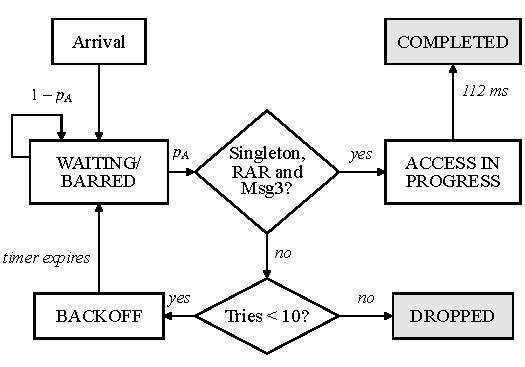
\includegraphics[width=3.5in]{figures/fig_lifecycle.pdf}
\caption{Life cycle of one request. Shaded states are terminal. A deadline miss is
recorded as a separate event and does not stop a request from being served.}
\label{fig:lifecycle}
\end{figure}

\subsection{Service and Conservation}
Let $c_i$ be the completion time of request $i$. Request $i$ is on time if it
completes at or before its deadline:
\begin{equation}
I_i =
\begin{cases}
1, & \text{if request $i$ completes and } c_i \le d_i,\\
0, & \text{otherwise.}
\end{cases}
\label{eq:ontime}
\end{equation}
A request that completes exactly at $d_i$ counts as on time. Late, dropped, and
unfinished requests all give $I_i = 0$. The primary metric is the on-time fraction
over the evaluable cohort $\mathcal{E}(H)$, which contains all requests whose
deadlines have elapsed by $H$ and any request dropped before its deadline:
\begin{equation}
P_{\mathrm{on}} = \frac{1}{|\mathcal{E}(H)|}
\sum_{i \in \mathcal{E}(H)} I_i.
\label{eq:pon}
\end{equation}
With the chosen horizon, $\mathcal{E}(H)$ contains every generated request, so
policies are scored on the same requests.

The simulator keeps a ledger in which, at all times $t$,
\begin{equation}
A(t) = C(t) + X(t) + B(t),
\label{eq:conservation}
\end{equation}
where $A$ counts generated requests, $C$ completed requests, $X$ dropped requests,
and $B$ requests still pending. During test evaluation the check runs at the end of
every decision window and a violation aborts the run. It shows correct accounting,
not good performance.

\subsection{Resource Budget}
Resources are counted in units of 3.75~kHz~$\times$~1~ms. In decision window $k$,
\begin{equation}
R_{\mathrm{RACH}}(k) + R_{\mathrm{DATA}}(k) \le R_{\mathrm{total}} = 30\,720,
\label{eq:resource}
\end{equation}
which corresponds to 48 subcarriers over 640~ms. NPRACH reserves $n \times 5.6$ units
per opportunity, using the format~0 preamble duration~\cite{ts36211}, and each Msg3
grant uses 6 units. At these values the largest NPRACH reservation is 1075 units, or
3.5\% of $R_{\mathrm{total}}$, so \eqref{eq:resource} is not a binding limit here. A
larger $n$ costs little in this model, and that should be remembered when judging the
value of NPRACH control in Section~\ref{sec:results}.

\subsection{Capacity Check}
The expected number of singletons per opportunity is at most $n(1-1/n)^{n-1}$, reached
when $n$ requests attempt. For $n = 48$ this is 17.9, or about 223 preamble successes
per second, which is below the RAR limit of 300 per second. At the Beta(3,4) mode the
event rate is 2.07 times its 10~s average, so total arrivals peak near $0.0115\,N$
requests per second, or about 344 per second at $N = 30\,000$. This peak exceeds the
access ceiling for $N$ above about 19\,400. Even so, a burst can drain afterward. At
the ceiling, net of the periodic rate, a first-order clearing time is 8~s at
$N = 30\,000$, 15~s at $50\,000$, 27~s at $75\,000$, and 45~s at $100\,000$. The tested
populations thus range from feasible to overloaded, and above roughly 80\,000 meters
no controller should be expected to serve the whole burst within 30~s.

\subsection{Problem Statement}
At the start of each 640~ms window $k$, the controller selects
$a_k = (p_A, b, n)$ from a feasible set $\mathcal{A}$ using only network-side
observations. The goal is a policy $\pi$ that solves
\begin{equation}
\max_{\pi}\ \mathbb{E}\big[P_{\mathrm{on}}(\pi)\big]
\quad \text{s.t.} \quad a_k \in \mathcal{A}\ \ \forall k,
\ \text{\eqref{eq:conservation}, \eqref{eq:resource}.}
\label{eq:problem}
\end{equation}
The expectation is over traffic and contention. Arrivals are unknown in advance,
requests are not individually visible to the controller, and each action affects
later congestion through retries. Deadlines therefore enter as a soft objective,
and no guarantee is implied.

\section{Proposed Controller}
\label{sec:controller}
The controller is a tabular Q-learning agent~\cite{watkins} at the eNodeB (eNB).
Fig.~\ref{fig:loop} shows its interaction with the cell, and Algorithm~1 gives the
procedure with the same step numbers. Within a window, steps (1) to (3) and (7) repeat
at each of the eight NPRACH opportunities, under the action chosen for that window.

\begin{figure}[!t]
\centering
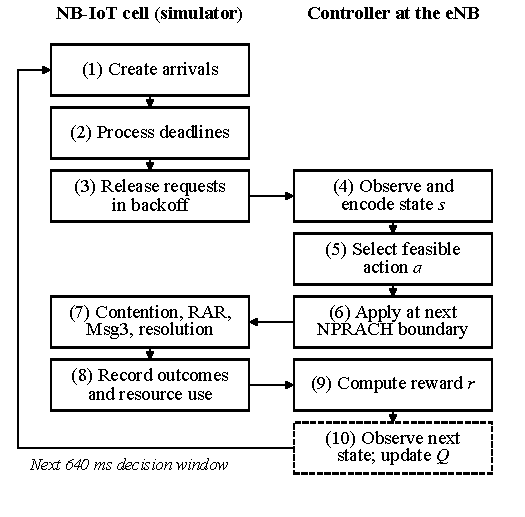
\includegraphics[width=3.5in]{figures/fig_control_loop.pdf}
\caption{Control and learning loop for one decision window. Step numbers match
Algorithm~1. The dashed step updates $Q$ during training only.}
\label{fig:loop}
\end{figure}

\subsection{Observation and State}
The controller sees only receiver-side counts for each opportunity: the number of
idle, occupied, and collided subcarriers. Treating these counts as exact is an
ideal-detection assumption. Three features are computed from them.

\emph{Congestion} is an exponentially weighted average, with weight 0.2, of collided
over occupied subcarriers. \emph{Load} starts from the idle-count estimate of the
number of attempting requests,
\begin{equation}
\hat{L} = \frac{1}{p_A}\,\frac{\ln(I/n)}{\ln(1-1/n)},
\label{eq:load}
\end{equation}
where $I$ is the idle count and $0 < I < n$. If $I = n$, then $\hat{L} = 0$; if $I = 0$,
the estimate saturates and is capped using $N$. The estimates are averaged over a
window and divided by 48. \emph{Trend} is the ratio of this window's load estimate
to the previous one.

The three features are quantized into 5, 5, and 6 bins, giving 150 states. Congestion
uses bins of width 0.2, load uses edges at 0, 1, 5, 20, 100, and $\infty$, and trend
uses edges at 0, 0.5, 0.8, 1, 1.25, 2, and $\infty$. This state is a quantized
observation of a partially observed process: it omits request ages and retry timers,
so the Markov property is not assumed, and the convergence result of~\cite{watkins}
does not directly apply.

\subsection{Actions}
The action set is the product of nine admission probabilities,
$p_A \in \{0.001, 0.005, 0.01, 0.025, 0.05, 0.1, 0.25, 0.5, 1\}$, four backoff
windows, $b \in \{0, 256, 1024, 4096\}$~ms, and the four values of $n$, giving
144 joint actions. The backoff values are NB-IoT table entries~\cite{ts36321}. The
action is applied at the next NPRACH boundary and governs the whole window. Actions
that violate \eqref{eq:resource} are masked, although with these values none are.

Here $p_A$ is an abstract admission probability. It is not the ACB procedure of any
release, and mapping it to real broadcast signaling remains open work.

\subsection{Reward}
After a window ends, the reward is computed from what actually happened in it:
\begin{equation}
r_k = \frac{w_{\mathrm{on}} C_{\mathrm{on}}
 - w_{\mathrm{miss}} M_{\mathrm{new}}
 - w_{\mathrm{drop}} X_{\mathrm{new}}}{K}
 - w_q B_{\mathrm{norm}} - w_r R_{\mathrm{norm}}.
\label{eq:reward}
\end{equation}
$C_{\mathrm{on}}$ counts requests that completed on time in the window, which is
the only positive term. $M_{\mathrm{new}}$ counts deadlines that matured in the window
for requests that will not complete on time and were not already dropped.
$X_{\mathrm{new}}$ counts new terminal drops. A request that misses its deadline and
is later dropped incurs both costs, since they are different failures, but each cost
is applied once.

$B_{\mathrm{norm}}$ is the pending count divided by $N$, a simulator signal used only
during training and never observed by the frozen controller. $R_{\mathrm{norm}}$ is
the window's resource use over $R_{\mathrm{total}}$. The scale $K = 384$ equals 48
choices over 8 opportunities and does not depend on the action, so the controller
cannot raise its reward by changing a denominator.

\subsection{Learning}
With state $s_k$, action $a_k$, and next state $s_{k+1}$ taken from the actual next
observation, the table is updated as
\begin{equation}
Q(s_k,a_k) \leftarrow Q(s_k,a_k) + \alpha
\big[ r_k + \gamma \max_{a' \in \mathcal{A}} Q(s_{k+1},a') - Q(s_k,a_k) \big],
\label{eq:qupdate}
\end{equation}
with no continuation term on the final window. The learning rate is
$\alpha = (1+v)^{-0.6}$, where $v$ is the visit count of the pair $(s_k,a_k)$, and
$\gamma = 0.99$, which is an effective horizon of about 64~s at one decision per
640~ms. Exploration is $\epsilon$-greedy, with $\epsilon$ falling linearly from 1.0 to
0.05 over the first 80\% of episodes. The table is initialized to zero. Every 200
episodes the greedy policy is scored on validation traces, and the best checkpoint
is kept and frozen with $\epsilon = 0$.

\begin{figure}[!t]
\footnotesize
\hrule\smallskip
\textbf{Algorithm 1:} Training and frozen-policy evaluation
\smallskip\hrule\smallskip
\begin{algorithmic}[0]
\REQUIRE Traffic model, action set $\mathcal{A}$, state encoder, reward weights
\STATE Initialize $Q(s,a) \leftarrow 0$
\FOR{each training episode}
  \STATE Reset simulator, ledger, timers, and counters
  \WHILE{the episode has not ended}
    \STATE (1) Create arrivals
    \STATE (2) Process matured deadlines
    \STATE (3) Release requests whose backoff timers expired
    \STATE (4) Observe measurements and encode state $s$
    \STATE (5) Select $a \in \mathcal{A}$ by $\epsilon$-greedy
    \STATE (6) Apply $a$ at the next NPRACH boundary
    \STATE (7) Simulate contention, RAR, Msg3, and resolution
    \STATE (8) Record outcomes and resource use
    \STATE (9) Compute $r$ using \eqref{eq:reward}
    \STATE (10) Observe next state $s'$; update $Q$ using \eqref{eq:qupdate}
  \ENDWHILE
\ENDFOR
\STATE Restore the best validation checkpoint; set $\epsilon \leftarrow 0$
\STATE Evaluate on held-out traces with no further updates, aborting if
\eqref{eq:conservation} fails
\end{algorithmic}
\smallskip\hrule
\end{figure}

\subsection{Controller Cost}
The table holds $150 \times 144$ single-precision values, or 86\,400 bytes, and a
frozen policy reduces to a 300-byte map from state to action. A greedy scan is
$O(|\mathcal{A}|)$, while the frozen map is a constant-time lookup. Training is
offline in the simulator. Over 20\,000 random states, a greedy scan took 4.6 to
5.0~$\mu$s per decision on a cloud Linux virtual machine running Python 3.11, which is
negligible against the 640~ms decision interval.

\section{Evaluation Methodology}
\label{sec:evaluation}
\subsection{Parameters}
Table~\ref{tab:params} lists the parameters. Values marked $\dagger$ are listed in
the 3GPP Release~15 specifications~\cite{ts36331}, \cite{ts36321}, \cite{ts36211},
and the rest are study assumptions.

\begin{table}[!t]
\caption{Simulation Parameters}
\label{tab:params}
\centering
\begin{tabular}{@{}l l@{}}
\hline
\textbf{Parameter} & \textbf{Value} \\
\hline
Meters $N$ & 10\,000 to 100\,000 (six values) \\
Training population & 30\,000 \\
Periodic report period, deadline & 900~s, 60~s \\
Event onset, spread, share of meters & 30~s, 10~s, 5\% \\
Event deadline & 30~s \\
Arrival window, horizon $H$ & 120~s, 180~s \\
NPRACH period, offset$^\dagger$ & 80~ms, 8~ms \\
Subcarriers $n^\dagger$ & 12, 24, 36, 48 \\
Preamble duration$^\dagger$ & 5.6~ms (format 0) \\
Backoff windows $b^\dagger$ & 0, 256, 1024, 4096~ms \\
Attempt limit & 10 \\
RAR grants per opportunity & 24 \\
Msg3 size & 6 resource units \\
RAR, Msg3, resolution delay & 40, 32, 40~ms \\
Decision interval & 640~ms \\
$w_{\mathrm{on}}, w_{\mathrm{miss}}, w_{\mathrm{drop}}$ & 1, 1, 1 \\
$w_q, w_r, K$ & 0.01, 0.01, 384 \\
\hline
\end{tabular}
\end{table}

\subsection{Compared Methods}
Table~\ref{tab:methods} lists the six methods. All use the same simulator, traces,
resource budget, and action values, and the same names are used throughout. B2 to B5
share one learner and differ only in which controls are free, so any difference
between them comes from the action set. A control that is not free is pinned to
$b = 0$ or $n = 48$. B0 is the best fixed action on validation traces at the training
population, from a 24-point grid of $p_A \in [0.01, 0.5]$ and the four $b$ values with
$n = 48$. The selected action is $p_A = 0.05$, $b = 0$, and $n = 48$, which served
every validation request on time. B1 is an adapted occupancy-matching heuristic in the
spirit of~\cite{duan}, not a reproduction of that algorithm. In every window it sets
$p_A$ to the grid value nearest to $\min(1, n/\hat{L})$, using the same load estimate
\eqref{eq:load} that the learned controllers observe, with $b = 0$ and $n = 48$. No
deep-RL baseline is evaluated, so this paper makes no comparison with deep RL.

\begin{table}[!t]
\caption{Compared Methods}
\label{tab:methods}
\centering
\begin{tabular}{@{}l l l@{}}
\hline
\textbf{ID} & \textbf{Method} & \textbf{Free controls} \\
\hline
B0 & Tuned fixed & None \\
B1 & Occupancy matching & $p_A$ (rule based) \\
B2 & Q-admission & $p_A$ \\
B3 & Q-admission+backoff & $p_A, b$ \\
B4 & Q-admission+NPRACH & $p_A, n$ \\
B5 & Q-joint (proposed) & $p_A, b, n$ \\
\hline
\end{tabular}
\end{table}

\subsection{Training and Testing}
Each learned method is trained for 2000 episodes at $N = 30\,000$ with five training
seeds, cycling through ten training traces. One episode has 282 decisions. Validation
uses eight separate traces. Frozen policies are then tested at all six populations
on twenty held-out traces that are shared across methods, so comparisons are paired.
Training at one population and testing at others also shows how far a policy
generalizes beyond its training load.

To test the reward design, B5 is retrained with two seeds under two alternatives to
\eqref{eq:reward}: a throughput-only reward that counts all completions, early or
late, and the deadline-aware reward without the backlog and resource terms.

\subsection{Metrics}
$P_{\mathrm{on}}$ in \eqref{eq:pon} is the primary metric, reported overall and for
event requests alone. Secondary metrics are the median, 95th percentile, and 99th
percentile of delay; drops; resource utilization; and preamble success, defined as
singleton preambles over transmitted preambles. Delay is measured from arrival to
completion for completed requests only, so it is always read alongside
$P_{\mathrm{on}}$. Collision is not reported separately: among transmitted preambles
it is the exact complement of preamble success and carries no new information. No
energy metric is reported, because no power model is implemented.

Each learned method is scored on 100 runs, five training seeds times twenty test
traces, and each of B0 and B1 on the twenty traces. Results are the mean and standard
deviation over these runs, and comparisons of $P_{\mathrm{on}}$ use its 95\% bootstrap
interval.

\subsection{Simulator Validation}
Automated tests cover conservation, deadline boundaries (including completion exactly
at $d_i$), the singleton count against its analytical mean, backoff, action timing,
resource accounting, reward event counting, the Q update, and reproducibility from a
fixed seed.

\section{Results and Discussion}
\label{sec:results}
All numbers in this section come from the frozen full-budget run described in
Section~\ref{sec:evaluation}; none come from pilot runs.

\subsection{Training and Validation}
Validation at the training population is close to its ceiling. The best checkpoint of
every one of the 20 learned runs scores between 0.989 and 1.000, and B0 scores 1.000.
For B2, B3, and B5, the mean validation $P_{\mathrm{on}}$ over seeds is highest within
the first 800 episodes and then falls by about 0.01 as $\epsilon$ decays, for example
from 0.994 to 0.984 for B5. B4 starts lower and peaks near episode 1000. Checkpoint
selection therefore keeps early policies: four of the 20 selected checkpoints come
from episode 200, when $\epsilon$ was still 0.88. Training visited 101 to 133 of the 150 states, and 30\% to 64\% of
the feasible state-action pairs, with the lowest share for B5, which has 144 actions
per state.

\subsection{Reference Load}
At $N = 30\,000$, every method serves more than 99\% of requests on time,
and B0 serves all of them (Table~\ref{tab:results}). The learned controllers
therefore do not improve on a tuned fixed action at the load they were trained on.
They differ in how they reach this level. B4 and B5 reserve fewer subcarriers and
lower resource utilization from 0.074 to 0.058 and 0.054, but their preamble success
falls from 0.79 to 0.55--0.57 and they drop about 40 requests per run. Because the
resource budget is far from binding in this model (Section~\ref{sec:model}), this
saving has little value here. B1 has the lowest tail delay but misses 2.8\% of event
requests.

\begin{table}[!t]
\caption{Performance at $N = 30\,000$ on Held-Out Traces}
\label{tab:results}
\centering
\begin{tabular}{@{}l c c c c c c@{}}
\hline
\textbf{ID} & $P_{\mathrm{on}}$ & $P_{\mathrm{on}}^{\mathrm{ev}}$ &
\textbf{p99 (s)} & \textbf{Drops} & \textbf{Preamble} & \textbf{Res.} \\
\hline
B0 & 1.000 & 1.000 & 9.27 & 0.0 & 0.794 & 0.074 \\
B1 & 0.992 & 0.972 & 4.39 & 46.4 & 0.603 & 0.074 \\
B2 & 0.998 & 0.993 & 7.13 & 13.6 & 0.684 & 0.074 \\
B3 & 1.000 & 0.999 & 8.55 & 1.7 & 0.734 & 0.074 \\
B4 & 0.993 & 0.979 & 11.14 & 40.5 & 0.554 & 0.058 \\
B5 & 0.993 & 0.979 & 10.18 & 36.8 & 0.573 & 0.054 \\
\hline
\multicolumn{7}{@{}p{3.3in}@{}}{Means over 100 runs (5 seeds $\times$ 20 traces) for
B2--B5 and 20 runs for B0 and B1; each run has 5511 requests. The standard deviation
over runs is at most 0.010 for $P_{\mathrm{on}}$ and 0.031 for
$P_{\mathrm{on}}^{\mathrm{ev}}$. $P_{\mathrm{on}}^{\mathrm{ev}}$: event requests only.
Drops: per run. Preamble: preamble success. Res.: resource utilization.}
\end{tabular}
\end{table}

\subsection{Load Sweep}
Figs.~\ref{fig:ontime} and~\ref{fig:event} show the frozen policies at all six
populations. Up to 30\,000 meters, where the capacity check of
Section~\ref{sec:model} predicts that a burst clears within about 8~s, all methods
serve at least 99\% of requests on time. The learned policies degrade as the load
moves away from the training value. At 50\,000 meters B0 still serves 99.7\%, while
the learned variants serve 89.4\% to 97.3\%. At 75\,000 meters, where the clearing
time approaches the 30~s event deadline, and at 100\,000 meters, where it exceeds
it, B1 serves 99.2\% and
96.1\% of all requests and 97.7\% and 86.8\% of event requests. The best learned
variant, B3, serves 86.3\% and 78.1\% overall and 59.9\% and 39.8\% of event requests.

The one-control and two-control variants show what each control adds. Adding
backoff to admission (B3 against B2) raises $P_{\mathrm{on}}$ at every population of
50\,000 and above, by 1.6 to 4.0 points, and event $P_{\mathrm{on}}$ by 7 to 12
points; at 100\,000 meters the bootstrap intervals of B3 and B2 do not overlap.
Adding NPRACH control lowers $P_{\mathrm{on}}$ instead: B4 is 3.9 to 6.1 points below
B2, and the joint controller B5 is 4.0 to 6.8 points below B3 over the same range.
The NPRACH policies learned at 30\,000 meters reserve fewer subcarriers, which costs
little at that load but removes contention capacity when the load is higher. Joint
control of all three variables therefore does not improve on-time service in this
study.

The contrast with B1 points to generalization rather than to the observation. B1
reads the same load estimate as the learned controllers, but its rule
$p_A \approx n/\hat{L}$ scales with load by construction. The tabular policies were
trained only at 30\,000 meters and act in high-load states that they visited rarely
or never during training.

\begin{figure}[!t]
\centering
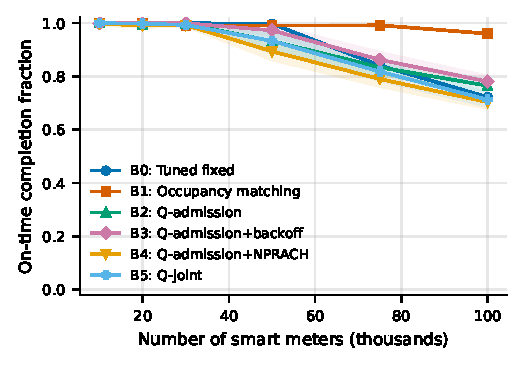
\includegraphics[width=3.5in]{figures/fig_on_time_vs_load.pdf}
\caption{On-time fraction versus number of meters on held-out traces. Lines are
means; shaded bands show $\pm 1$ standard deviation over runs for the learned
methods.}
\label{fig:ontime}
\end{figure}

\begin{figure}[!t]
\centering
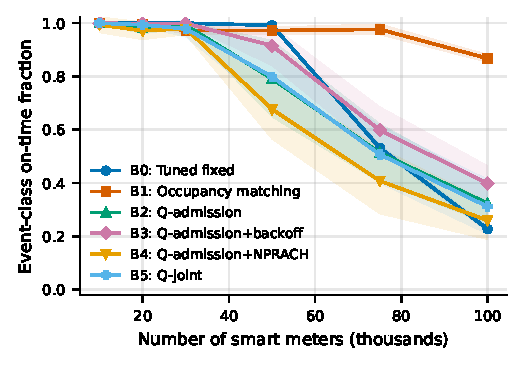
\includegraphics[width=3.5in]{figures/fig_on_time_event_vs_load.pdf}
\caption{On-time fraction of event requests versus number of meters.}
\label{fig:event}
\end{figure}

\subsection{Tail Delay}
Fig.~\ref{fig:p99} must be read together with Fig.~\ref{fig:ontime}, because the
delay of completed requests ignores the requests that never completed. B0 has a p99
delay of 7.7~s even at 10\,000 meters, since its fixed $p_A = 0.05$ holds requests
back when there is no congestion. At 75\,000 meters and above, B2 has the lowest p99
delay, about 16.6~s, while serving only 83.4\% and 76.5\% of requests on time. B1 has
the highest p99 delay at 100\,000 meters, 37.4~s, because it completes many requests
late in the burst that the other methods fail to complete at all. Low tail delay is
therefore not evidence of good service here.

\begin{figure}[!t]
\centering
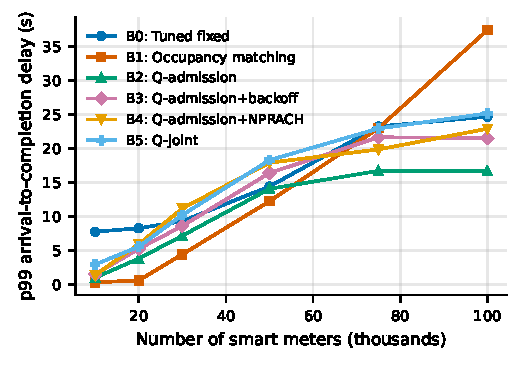
\includegraphics[width=3.5in]{figures/fig_p99_delay_vs_load.pdf}
\caption{99th-percentile delay of completed requests versus number of meters.}
\label{fig:p99}
\end{figure}

\subsection{Reward Ablation}
At $N = 30\,000$, B5 trained with the full reward \eqref{eq:reward} serves 99.5\% of
requests and 98.5\% of event requests on time (mean of two seeds). With the
throughput-only reward these fall to 96.2\% and 87.9\%, and drops rise from 26 to 207
per run, even though the p99 delay is lower, 8.0~s against 10.5~s. Removing the
backlog and resource terms gives 99.6\% and 98.7\%, which is no measurable change.
The deadline terms therefore carry the benefit of the reward design, and the two
penalty terms have no visible effect at this load. With two seeds, and one
throughput-only seed reaching a best validation score of only 0.94, these
differences indicate direction rather than size.

\subsection{Limits}
The results apply to the stated simulation model. It has one cell, one coverage group,
and ideal reception, and it does not represent signaling for dynamic reconfiguration or
application-layer delivery. The state ablation, the reward-weight sensitivity, and
held-out event scenarios were not part of this evaluation. The learned policies were
trained at a single population, and training left 36\% to 70\% of the feasible
state-action pairs unvisited; the frozen policy has no learned preference there. The
widening gap to B1 as the load moves away from 30\,000 meters is consistent with this,
and training across several populations is the most direct next test. Validation at
the training population is near its ceiling, so it separates checkpoints only weakly.

\section{Conclusion}
The deadline terms of the reward matter: without them, the same learner's on-time
service for event requests falls from 98.5\% to 87.9\%. Joint learned control of admission,
backoff, and NPRACH configuration, however, did not improve on-time service over a
tuned fixed action at the training load, and away from that load it fell well
behind a simple load-matching rule that uses the same observation. Of the three
controls, backoff added the most; NPRACH control saved resources that were not
scarce and cost on-time service at higher loads. For tabular learning in this
setting, how the controller generalizes across load matters more than how many
controls it coordinates. Future work should train across populations and map the admission control to real NB-IoT signaling, add
channel and coverage effects, and test other event shapes and deadlines before any
deployment conclusion is drawn.

\section*{Acknowledgment}
\ifblind\else
\pending{funding and support, including Genus Power Infrastructures Ltd.}
\fi
The simulator code, a first draft of this manuscript, and the scripts that draw
Figs.~\ref{fig:lifecycle} and~\ref{fig:loop} were prepared with Claude (Anthropic).
\pending{Authors: confirm or correct this statement, and name any other tools and
sections.} The authors reviewed this material and take full responsibility for the
content of this paper.

\begin{thebibliography}{00}
\bibitem{wang} Y.-P. E. Wang \emph{et al.}, ``A primer on 3GPP narrowband Internet of Things,'' \emph{IEEE Commun. Mag.}, vol. 55, no. 3, pp. 117--123, Mar. 2017, doi: 10.1109/MCOM.2017.1600510CM.
\bibitem{stusek} M. Stusek \emph{et al.}, ``Exploiting NB-IoT network performance and capacity for smart-metering use-cases,'' in \emph{Proc. 15th Int. Congr. Ultra Mod. Telecommun. Control Syst. Workshops (ICUMT)}, Oct. 2023, pp. 193--199, doi: 10.1109/ICUMT61075.2023.10333294.
\bibitem{abbas} A. M. Abbas, K. Y. Youssef, I. I. Mahmoud, and A. Zekry, ``NB-IoT optimization for smart meters networks of smart cities: Case study,'' \emph{Alexandria Eng. J.}, vol. 59, no. 6, pp. 4267--4281, Dec. 2020, doi: 10.1016/j.aej.2020.07.030.
\bibitem{laya} A. Laya, L. Alonso, and J. Alonso-Zarate, ``Is the random access channel of LTE and LTE-A suitable for M2M communications? A survey of alternatives,'' \emph{IEEE Commun. Surveys Tuts.}, vol. 16, no. 1, pp. 4--16, 1st Quart., 2014, doi: 10.1109/SURV.2013.111313.00244.
\bibitem{iiyambo} L. Iiyambo, G. Hancke, and A. M. Abu-Mahfouz, ``A survey on NB-IoT random access: Approaches for uplink radio access network congestion management,'' \emph{IEEE Access}, vol. 12, pp. 95487--95506, 2024, doi: 10.1109/ACCESS.2024.3419216.
\bibitem{duan} S. Duan, V. Shah-Mansouri, Z. Wang, and V. W. S. Wong, ``D-ACB: Adaptive congestion control algorithm for bursty M2M traffic in LTE networks,'' \emph{IEEE Trans. Veh. Technol.}, vol. 65, no. 12, pp. 9847--9861, Dec. 2016, doi: 10.1109/TVT.2016.2527601.
\bibitem{tello} L. Tello-Oquendo, D. Pacheco-Paramo, V. Pla, and J. Martinez-Bauset, ``Reinforcement learning-based ACB in LTE-A networks for handling massive M2M and H2H communications,'' in \emph{Proc. IEEE Int. Conf. Commun. (ICC)}, May 2018, pp. 1--7, doi: 10.1109/ICC.2018.8422167.
\bibitem{pacheco} D. Pacheco-Paramo, L. Tello-Oquendo, V. Pla, and J. Martinez-Bauset, ``Deep reinforcement learning mechanism for dynamic access control in wireless networks handling mMTC,'' \emph{Ad Hoc Netw.}, vol. 94, Nov. 2019, Art. no. 101939, doi: 10.1016/j.adhoc.2019.101939.
\bibitem{hadjadj} Y. Hadjadj-Aoul and S. Ait-Chellouche, ``Access control in NB-IoT networks: A deep reinforcement learning strategy,'' \emph{Information}, vol. 11, no. 11, Nov. 2020, Art. no. 541, doi: 10.3390/info11110541.
\bibitem{sharma} S. K. Sharma and X. Wang, ``Collaborative distributed Q-learning for RACH congestion minimization in cellular IoT networks,'' \emph{IEEE Commun. Lett.}, vol. 23, no. 4, pp. 600--603, Apr. 2019, doi: 10.1109/LCOMM.2019.2896929.
\bibitem{jiang19} N. Jiang, Y. Deng, A. Nallanathan, and J. A. Chambers, ``Reinforcement learning for real-time optimization in NB-IoT networks,'' \emph{IEEE J. Sel. Areas Commun.}, vol. 37, no. 6, pp. 1424--1440, Jun. 2019, doi: 10.1109/JSAC.2019.2904366.
\bibitem{jiang21} N. Jiang, Y. Deng, A. Nallanathan, and J. Yuan, ``A decoupled learning strategy for massive access optimization in cellular IoT networks,'' \emph{IEEE J. Sel. Areas Commun.}, vol. 39, no. 3, pp. 668--685, Mar. 2021, doi: 10.1109/JSAC.2020.3018806.
\bibitem{bui} A.-T. H. Bui and A. T. Pham, ``Deep reinforcement learning-based access class barring for energy-efficient mMTC random access in LTE networks,'' \emph{IEEE Access}, vol. 8, pp. 227657--227666, 2020, doi: 10.1109/ACCESS.2020.3045811.
\bibitem{alcaraz} J. J. Alcaraz, J.-C. Sanchez-Aarnoutse, A.-S. Martinez-Sala, and F.-J. Gonzalez-Casta\~{n}o, ``Random access control in NB-IoT with model-based reinforcement learning,'' \emph{IEEE Internet Things J.}, vol. 12, no. 7, pp. 8135--8149, Apr. 2025, doi: 10.1109/JIOT.2024.3499854.
\bibitem{mehri} H. Mehri, H. Mehrpouyan, and H. Chen, ``RACH traffic prediction in massive machine type communications,'' \emph{IEEE Trans. Mach. Learn. Commun. Netw.}, vol. 3, pp. 315--331, 2025, doi: 10.1109/TMLCN.2025.3542760.
\bibitem{martiradonna} S. Martiradonna, G. Piro, and G. Boggia, ``On the evaluation of the NB-IoT random access procedure in monitoring infrastructures,'' \emph{Sensors}, vol. 19, no. 14, Jul. 2019, Art. no. 3237, doi: 10.3390/s19143237.
\bibitem{caso} G. Caso, K. Kousias, \"{O}. Alay, A. Brunstrom, and M. Neri, ``NB-IoT random access: Data-driven analysis and ML-based enhancements,'' \emph{IEEE Internet Things J.}, vol. 8, no. 14, pp. 11384--11399, Jul. 2021, doi: 10.1109/JIOT.2021.3051755.
\bibitem{ts36331} \emph{LTE; Evolved Universal Terrestrial Radio Access (E-UTRA); Radio Resource Control (RRC); Protocol Specification}, ETSI TS 136 331 V15.3.0 (3GPP TS 36.331 Version 15.3.0 Release 15), ETSI, Sophia Antipolis, France, Oct. 2018.
\bibitem{tr37868} \emph{Study on RAN Improvements for Machine-Type Communications}, 3GPP TR 37.868 V11.0.0, 3GPP, Sophia Antipolis, France, Sep. 2011.
\bibitem{ts36211} \emph{LTE; Evolved Universal Terrestrial Radio Access (E-UTRA); Physical Channels and Modulation}, ETSI TS 136 211 V15.3.0 (3GPP TS 36.211 Version 15.3.0 Release 15), ETSI, Sophia Antipolis, France, Oct. 2018.
\bibitem{watkins} C. J. C. H. Watkins and P. Dayan, ``Technical note: Q-learning,'' \emph{Mach. Learn.}, vol. 8, no. 3--4, pp. 279--292, May 1992, doi: 10.1023/A:1022676722315.
\bibitem{ts36321} \emph{LTE; Evolved Universal Terrestrial Radio Access (E-UTRA); Medium Access Control (MAC) Protocol Specification}, ETSI TS 136 321 V15.3.0 (3GPP TS 36.321 Version 15.3.0 Release 15), ETSI, Sophia Antipolis, France, Oct. 2018.
\end{thebibliography}

\end{document}
